\documentclass[tc]{copernicus}

\usepackage{booktabs}
\usepackage{multirow}
\usepackage{siunitx} 

\begin{document}
\nolinenumbers

\title{Artificial ice reservoirs research direction}

\def\Authors{Suryanarayanan Balasubramanian\,$^{1,2}$}

\def\corrAuthor{Suryanarayanan Balasubramanian}
\Author[1,2]{Suryanarayanan}{Balasubramanian}
\Author[1]{Martin}{Hoelzle}
\affil[1]{University of Fribourg, Department of Geosciences, Fribourg, Switzerland}
\affil[2]{Himalayan Institute of Alternatives, Ladakh, India}

\correspondence{gayashiva91@gmail.com}

\runningtitle{Artificial ice reservoirs}

\runningauthor{S. Balasubramanian}

\firstpage{1}

\maketitle

\section{Summary}

Irrigation networks in arid mountain regions are completely dependant on the timely availability of meltwater
from glaciers, snow and permafrost. With the accelerated decline of glaciers, these irrigation networks can no
longer deliver adequate water to sustain agricultural output and take advantage of the complete growing season.
As a consequence, some mountain villages have either been abandoned or lie on the brink of desertification
\citep{grossmanHimalayanGlaciersMelt2015}.

To cope with this recurrent water scarcity, villagers have developed two types of artificial ice reservoirs
(AIRs): ice stupas and ice terraces (see Fig. \ref{fig:AIRforms}). Both the ice reservoirs capture water in the
autumn and winter, allowing it to freeze, and hold it until spring, when it melts and flows down to the fields
\citep{ipccChapterHighMountain2019, vinceGlacierMan2009, clouseLadakhArtificialGlaciers2017,
nusserSociohydrologyArtificialGlaciers2019}. In this way, they retain a previously unused portion of the annual
flow and facilitate its use to supplement the decreased flow during the following spring.

\begin{figure}[t]
\centering
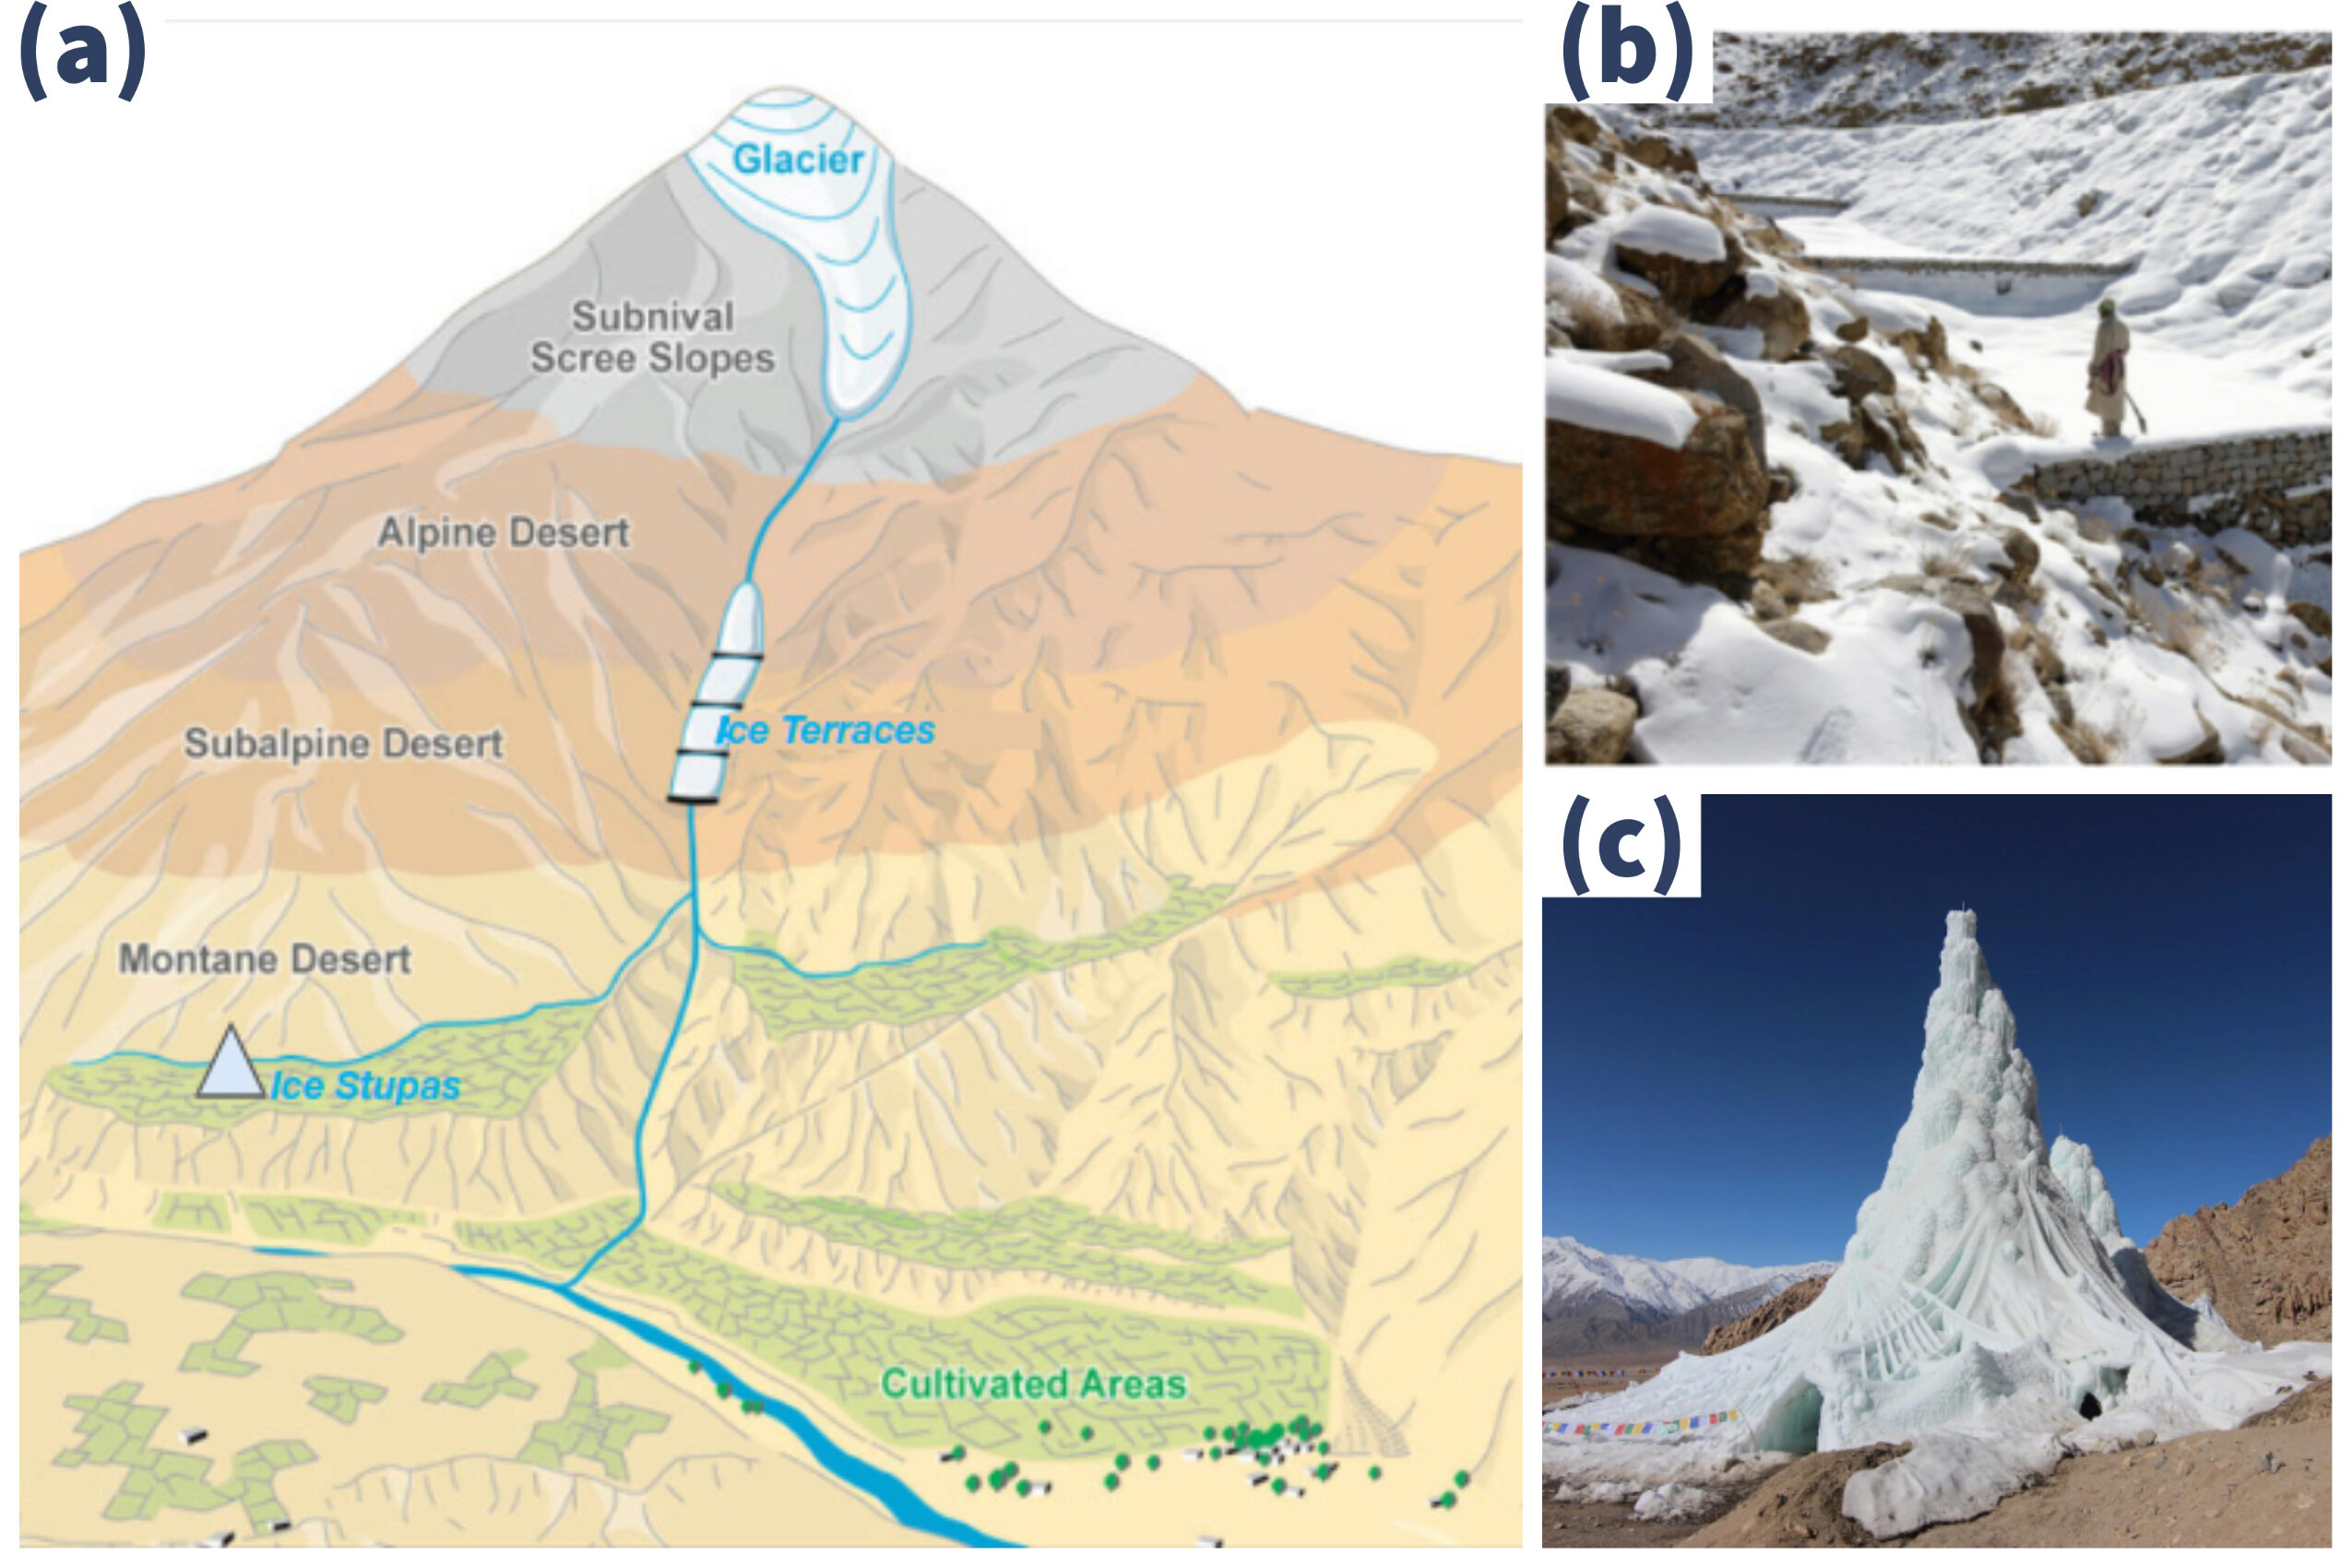
\includegraphics[width=\columnwidth]{figs/AIR_forms.jpg}

\caption{(a) Schematic overview of the position of artificial ice reservoirs. These constructions are located at
  altitudes between the glaciers and the irrigation networks in the cultivated areas. (b) Ice terraces at 3900
  m, located above the village of Nang, Ladakh. The cascade is composed of a series of loose masonry walls
  ranging in height from 2 to 3 $m$, which help freeze water for storage. (c) Ice stupas at 3600 m, located
above the village of Phyang, Ladakh. They are made using fountain systems. Adapted from:
\cite{nusserLocalKnowledgeGlobal2016}}

\label{fig:AIRforms}
\end{figure}

AIR observations and investigations date back to the mid-2000s \citep{tveitenGlacierGrowingLocal2007}. The vast
majority have been published in the 2010s, mostly using qualitative methods. However, quantifications of their
storage capacity differ widely amongst these publications \citep{baglaArtificialGlaciersHelp1998,
norphelSnowWaterHarvesting2015, nusserSociohydrologyArtificialGlaciers2019}. Because small-scale processes,
complex feedbacks and non-linearities govern their evolution, modelling the volume evolution of ice stupas is
only feasible if backed up with comprehensive input, calibration and validation datasets.

In response, we conducted measurement campaigns using drones, flowmeters and weather stations on 23 AIRs across
two locations (India and Switzerland), over four winters (2019, 2020, 2021 and 2022) and using two different
construction methods (traditional and automated). Each dataset contained information on the meteorological
conditions, fountain characteristics and AIR volume evolution. 

In \citet{balasubramanianInfluenceMeteorologicalConditions2022}, an AIR model was designed to resolve surface
processes and used to compare their volume evolution in Indian Himalayas and the Swiss Alps. In
\citet{balasubramanianFountainSchedulingStrategies2022}, the evolution of AIRs using different fountain
scheduling strategies were compared.  The results of these papers can be summarised as follows:

\begin{enumerate} 

\item Volumes of ice stupas located in different regions may differ by an order of magnitude. The differences
  could be attributed to the accelerated sublimation process in colder and drier regions.

\item Water losses of ice stupas may be upto 80 \% due to excessive water input. However, water supply
  management through fountain scheduling strategies can produce icestupas of similar volumes while reducing upto
  one-tenth of their water supply.

\item Traditional construction systems demand significant maintenance efforts since they are prone to freezing
  events in the fountain pipeline. However, automated construction systems can prevent these events to make the
  construction process maintenance-free.
\end{enumerate}


\section{Future research priorities}

Currently, no decision framework exists to design AIRs based on the water requirement of the respective mountain
catchments. However, AIR meltwater characteristics show significant potential for climate change adaptation
against reduced glacial water supply. For example, ice terraces near the Stok catchment in Ladakh have been
measured with areas upto 19 \% of the Stok glacier \citep{nusserSociohydrologyArtificialGlaciers2019,
sohebMassbalanceObservationReconstruction2020}. Therefore, AIRs can be an important tool to make mountain water
resource management resilient against hazards caused by vanishing glaciers, drying springs and shifts in
precipitation patterns. However, their applicability needs to be quantified across all mountain catchments
reliant on their glacial meltwater supply to understand the scope and potential of this water storage
technology.

Insights from our research could contribute to efforts to better estimate the future potential of AIRs for
climate change adaptation and mitigation under multiple plausible future climatic, demographic, economic, and
land use scenarios. 

\subsection{Quantification and development of ice terraces}

Although much focus is given to ice stupas, their ice volumes pale in comparison with ice terraces . For
example, ice terraces have attained volumes upto 30 times larger than ice stupas built in Ladakh, India
\citep{nusserSociohydrologyArtificialGlaciers2019}. This is because ice stupas are limited by their fountain's
spray radius. However, ice terraces have no such limitations. Their thickness is only limited by the water
supply rate or weather conditions and they can occupy any construction area provided. But despite this, ice
stupas are the preferred method of ice harvesting due to their longer survival duration and reduced construction
effort.

With a suitable redesign of the automation hardware, automated construction strategies can also be applied on
ice terraces. Such a construction strategy can potentially compound their size every consecutive winter with
minimal maintenance requirements. Therefore, future research direction should aim to answer the following
questions:

\begin{itemize}

  \item How can ice terrace construction systems be engineered to reduce their water losses and maintenance
    efforts?

\end{itemize}

\subsection{Quantifying sustenance of glacierized catchments with AIRs}

Glaciers provide an important buffer for highly seasonal precipitation regimes
\citep{kaserContributionPotentialGlaciers2010}. Under the currently available climate change projections it is
expected that glacial mass loss will continue in future decades, and that several smaller glaciers will continue
to disapear completely \citep{rabatelCurrentStateGlaciers2013}. 

In arid and semiarid regions, in particular, it is estimated that between 50 \% and 90 \% of freshwater
resources originate from mountain catchments \citep{messerliMountainsWorldVulnerable2004}. During drought
conditions in the tropical mountain regions, glacial meltwater is used by upto 3.92 million domestic users and
to irrigate 2096 $km^2$ of land \citep{buytaertGlacialMeltContent2017}.  

These trends stress the importance of increased water storage capacity for glacierized catchments as a pathway
for climate adaptation. Because of the challenges and cost related to traditional storage efforts, AIRs can be
a better tool to adapt against reduced glacial runoff. In order to quantify their adaptation potential, it
is necessary to understand the changing dynamics of AIR melting, but also map how their meltwater contributes to
current and future water use. While the spatiotemporal dynamics of AIR melt are increasingly well understood and
documented in \citet{balasubramanianInfluenceMeteorologicalConditions2022}, major uncertainty remains on how
their meltwater contribution propagates through the hydrological system and compares against the total discharge
of mountain catchments. 

Future research needs to determine which catchments can benefit most from the supplementary water supply
provided by these ice harvesting technologies and flag off the urgent climate action required to increase their
water security.

\bibliographystyle{copernicus}
\bibliography{zot_refs.bib}

\end{document}
